\documentclass[12pt]{TDTP}


\newcommand{\auteur}{C\'edric Lemaitre}
\newcommand{\couriel}{c.lemaitre58@gmail.com}
\newcommand{\promo}{Bachelor in Computer Vision}
\newcommand{\annee}{2017-2018}
\newcommand{\matiere}{Computer Aided Design 1}

\newcommand{\tdtp}{Practice}
\renewcommand{\sujet}{Intro to Matlab}


\begin{document}
\titre

\textbf{NOTE}\\
For each problem you shall create a script, for example \texttt{problem1.m}, containing all commands to answer the questions.

%%%%%%%%%%%%
\Exo
Make the following variables
\begin{enumerate}
\item $a = \begin{bmatrix} 3.14 \; 15 \; 9 \; 26 \end{bmatrix}$
\item $b = \begin{bmatrix} 2.71 \\ 7 \\ 2.1 \\ 71\\ \end{bmatrix}$
 \item $c = \begin{bmatrix} 5 \\ 4.8 \\ \vdots \\ -4.8\\ -5 \\ \end{bmatrix}$ (all the numbers from 5 to -5 in increments of -0.2).
 \item $A = \begin{bmatrix} 
 2 & \ldots & 2 \\ 
 \vdots & \ddots & \vdots\\ 
 2 & \ldots & 2 \\
 \end{bmatrix}$ a $9\times 9$ matrix full of 2's (use the commands \textbf{ones} or \textbf{zeros})
\item $B = \begin{bmatrix} 
 1 & 0 & \ldots & & 0 \\ 
 0 & \ddots & 0 \ddots & \\ 
 \vdots & 0 & 5 & 0 & \vdots \\
  & \ddots & 0 & \ddots & 0 \\
  0 &  & \ldots & 0 & 1\\
 \end{bmatrix}$ 
 a $9\times 9$ matrix of all zeros, but with the values $[1 \; 2 \; 3 \;  4 \; 5 \;  4 \;  3 \;  2 \;  1]$ on the main diagonal, use \textbf{zeros} and \textbf{diag}.
\item $C = \begin{bmatrix} 
 1 & 11 & \ldots & 91 \\ 
2 & 12 & \ldots & 92 \\ 
\vdots & \vdots & \ddots & \vdots \\ 
10 & 20 & \ldots & 100 \\ 
 \end{bmatrix}$
 a $10\times 10 $ matrix where the vector 1:100 runs down the columns (use \textbf{reshape})
 \item Create a $5\times 5$ matrix $D$ of random integers with values on the range -3 to 3. Use \textbf{rand} and \textbf{floor} or \textbf{ceil}.
\end{enumerate}

%%%%%%%%%%%%
\Exo
Solve the following equations using the variables created in \textbf{Problem 1}.
\begin{enumerate}
\item $x = \frac{1}{\sqrt{2\pi 2.5^2}} e^{-a^2/(2*2.5^2)}$
\item $y = \sqrt{(a^T)^2 + b^2}$
\item $z = \log_{10}(1/c) $, remember that $\log_{10}$ is the log base 10. So you use \textbf{log10} function. 
\end{enumerate}
Note that each of these variables is a vector of the right dimension.

%%%%%%%%%%%%
\Exo
If a matrix $A$ is defined using the MATLAB code $A=[1\; 3\; 2; \; 2\;1\;1; \; 3\; 2\; 3]$, which command will produce the following matrix
$$
B=\begin{bmatrix}
3&2\\
2&1\\
\end{bmatrix}
$$ 

%%%%%%%%%%%%
\Exo
Create the variables representing the following matrices:
$$
A=\begin{bmatrix}
1&2&3\\
2&2&2\\
-1&2&1\\
\end{bmatrix} \;\;
B=\begin{bmatrix}
1&0&0\\
1&1&0\\
1&1&1\\
\end{bmatrix} \;\;
C=\begin{bmatrix}
1&1\\
2&1\\
1&2\\
\end{bmatrix}
$$
\begin{itemize}
\item Try performing the following operations: $A+B$, $A*B$, $A+C$, $B-A$, $A*C$, $C-B$, $C*A$.
What are the results? What error messages are generated? Why?

\item What is the difference between $A*B$ and $A.*B$?
\end{itemize}

%%%%%%%%%%%%
\Exo
All points with coordinates $x=r\cos(\theta)$ and $y=\cos(\theta)$, where $r$ is a constant, lie on a circle with radius $r$. That is they satisfy the equation $x^2+y^2=r^2$.

Create a column vector for $\theta$ with the values, $0$, $\pi/4$, $\pi/2$, $3\pi/4$, and $5\pi/4$.
Take $r=2$ and compute the column vectors $x$ and $y$.

Now check that $x$ and $y$ indeed satisfy the equation of a circle, by computing the radius $r=\sqrt{(x^2+y^2)^2}$.

%%%%%%%%%%%%
\Exo
The sum of geometric series $1+r+r^2+r^3 + \cdots + r^n$, approaches the limit $\frac{1}{1-r}$ for $r<1$ as $n\rightarrow \infty$.

Take $r=0.5$ and compute the sums of series 0 to 10, 0 to 50, and 0 to 100.
Calculate the aforementioned limit and compare with your summations. Use the built-in \textbf{sum} function.

%%%%%%%%%%%%
\Exo
The number of ways to choose $k$ objects form a set of $n$ objects is defined and calculated with the formula
$$
\begin{pmatrix}
n\\k\\
\end{pmatrix}
= \dfrac{n!}{k!(n-k)!}
$$
Define a Pascal matrix with the formula 
$$
P(i,j) = \begin{pmatrix} i+j-2 \\ i-1\\ \end{pmatrix},
$$
where $i$ ranges from 1 to the number of rows and $j$ ranges from 1 to the number of columns.

Use this definition and hand calculations to find a Pascal matrix of dimension $4\times 4$.

Use Matlab's \textbf{pascal} command to check your result. 

%%%%%%%%%%%%
\Exo
Read the documention of MATLAb's \textbf{primes} command, and use it to store the first 100 primes less than or equal to 1000.
\begin{itemize}
\item Fin the sum of the first primes
\item Find the sum of the first, 20th and 97th primes.
\end{itemize}

%%%%%%%%%%%%
\Exo
Find a MATLAB one-line expression to cretae the $n\times n$ matrix $A$ satisfying
$$
a_{ij} = 
\begin{cases}
   1 & \text{if } i-j \text{ is prime} \\
   0  & \text{otherwise}
 \end{cases}
$$
%%%%%%%%%%%%
\Exo
\textbf{Manipulating variables}\\
For this problem, you need the file \emph{classGrades.mat}.
\begin{itemize}
\item Open a script and name it \emph{calculateGrades.m}. You'll write all the following command in this script.
\item Load the \emph{classGrades} file using the command \textbf{load}.
The file contains a single variable called \emph{namesAndGrades}.
\item To see how \emph{namesAndGrades} is structured, display the first 5 rows on your screen.
The first column contains the students 'names', they are just integers from 1 to 15.
The remaining 7 columns contain each student's score (on a sclae from 0 to 5) on each of 7 assignments.
There are also some NaNs which indicates that a particular student was absent on that day and didn't do the assignment.

\item We only care about the grades, so extract the submatrix containing all the rows but only columns 2 to 8 and name this new matrix \emph{grades}. To make this work for any size matrix, don't hard-code the 8, but rather use \textbf{end} or \textbf{size} commands. 
\end{itemize}

\begin{enumerate}
\item Calculate the mean score on each assignment. The result should be a 1x7 vector containing the mean grade on each assignment.

First, do this using \textbf{mean} and display the mean grades you get. What's wrong with this result?

Then use the \textbf{nanmean} command. What's different?

Name this mean vector \emph{meanGrades} (here you shoul use the vector without NaNs entries).

\item Now normalize each assignment so that the mean grade is 3.5. You'll want to divide each column of \emph{grades} by the correct element of \emph{meanGrades}.
\begin{itemize}
\item Make a matrix called \emph{meanMatrix} such that it is the same size as \emph{grades}, and each row has the values \emph{meanGrades}. 
\item Calculate the curved grades as $curvedGrades = 3.5 (grades/meanMatrix)$.
Keep in mind that you want to do the division elementwise.
\item Compute and display the mean of \emph{curvedGrades} to verify that they are all 3.5.
\item Because we divided by the mean and multiply by 3.5, it's possible that some grades that were initially close to 5 are now larger than 5.
To fix this, find all the elements in \emph{curvedGrades} that are greater than 5 and set them to 5. Use \textbf{find} command.
\end{itemize}

\item Calculate the total grade of each student and assign letter grades
\begin{itemize}
\item To calculate the \textit{totalGrade} vector, which will contain the numerical grade for each student, you want to take the mean of \textit{curvedGrades} across the columns (use \textbf{nanmean}, see help for how to specify the dimension). 
Also, we only want to end up with numbers from 1 to 5, so calculate the ceiling of the \textit{totalGrade} vector (use \textbf{ceil}).

\item Make a string called \textit{letters} that contains the letter grades in increasing order: FDCBA

\item Make the final letter grades vector \textit{letterGrades} by using \textit{totalGrade} (which should only contain values between 1 and 5) to index into \textit{letters}.

\item Finally, display the students grade using \textbf{disp}. You should find BCBBBACCBCCCCAB.
\end{itemize}
\end{enumerate}

%%%%%%%%%%%%
\Exo
\textbf{Friday  the 13th}\\
Friday the 13th is unlucky (in many cultures), but is it unlikely?
What's the probability that the 13th day of any month falls on a Friday?
The quick answer is 1/7, but this is not quite right.

Write a MATLAB code that counts the number of times that Friday occurs on the various weekdays in a 400 year Gregorian calendar cycle, for example from the year 1601 to the yera 2000.

\bigskip
\textbf{NOTE}:\\
The MATLAB function \textbf{clock} returns a six-element vector $c$ with elements
\begin{verbatim}
c(1) = year
c(2) = month
c(3) = day
c(4) = hour
c(5) = minute
c(6) = seconds
\end{verbatim}

The first five elements are integers, while the sixth element has a fractional part that is accurate to milliseconds. 
The best way to print a \textbf{clock} vector is to use \textbf{fprintf} or \textbf{sprintf} with a specified format string that has both integer and floating point fields.

\begin{verbatim}
f = '%6d %6d %6d %6d %6d %9.3f\n'
\end{verbatim}

On September 10th, 2014 at 3:15 pm, the following commands

\begin{verbatim}
c = clock;
fprintf(f,c);
\end{verbatim}

produces

\begin{verbatim}
2014	9	10	15	15	30.543
\end{verbatim}

In otrher words,

\begin{verbatim}
year = 2014
month = 9
day = 10
hour = 15
minute = 15
seconds = 30.543
\end{verbatim}

The MATLAB functions \textbf{datenum}, \textbf{datevec}, \textbf{datestr}, and \textbf{weekday} use \textbf{clock} and facts about the Gregorian calendar to facilitate computations involving calendar dates.
You migh want to use them to solve the problem.

%%%%%%%%%%%%
\Exo
Given the following function
$$
s = a \cos(\phi) + \sqrt{b^2 - (a\sin(\phi)-c)^2}
$$
Plot $s$ as a function of the angle $\phi$ when $a=1$, $b=1.5$, $c=0.3$, and $0\leq \phi \leq 360°$.

%%%%%%%%%%%%
\Exo
Plot the following parametric functions (you will use the \textbf{axis equal }command after your \textbf{plot} command to force MATLAB to make the x-axis and y-axis the same lenght):
\begin{itemize}
\item A circle of radius 5
\item \textit{Leminscate} ($-\pi/4 \leq \phi \leq \pi/4$)
\begin{align*}
x &= \cos(\phi) \sqrt{2\cos(2\phi)} \\
y &= \sin(\phi) \sqrt{2\cos(2\phi)}
\end{align*}

\item \textit{Logarithmic Spiral} ($0 \leq \phi \leq 6\pi; \; k=0.1$)
\begin{align*}
x &= e^{k\phi}\cos(\phi) \\
y &= e^{k\phi}\sin(\phi) 
\end{align*}

\end{itemize}
%%%%%%%%%%%%
\Exo
Plot the following 3D curves using \textbf{plot3} function:
\begin{itemize}
\item \textit{Spherical helix}
\begin{align*}
x &= \sin(\frac{t}{2c}) \cos(t) \\
y &= \sin(\frac{t}{2c}) \sin(t) \\
z &= \cos(\frac{t}{2c})
\end{align*}
where $c=5$ and $0\leq t \leq 10\pi$.

\item \textit{Sine wave on a sphere}
\begin{align*}
x &= \cos(t) \sqrt{b^2 -c^2 \cos^2(at)} \\
y &= \sin(t) \sqrt{b^2 -c^2 \cos^2(at)} \\
z &= c*\cos(at)
\end{align*}
where $a=10$, $b=1$, $c=0.3$, and $0 \leq t \leq 2\pi$.
\end{itemize}

%%%%%%%%%%%%
\Exo
Write a function to return the index of the value that is nearest to a desired value.
The function declaration should be
\begin{verbatim}
ind = findNearest(x, desiredVal)
\end{verbatim}
where $x$ is a vector or matrix of values, and \texttt{desiredVal} is the scalar value you want to find.

Do not assume that \texttt{desiredVal} exist in $x$, rather find the value that is closest to \texttt{desiredVal}.
Useful functions are \textbf{abs}, \textbf{min}, and \textbf{find}.
%%%%%%%%%%%%
\Exo
Write a function that implements the quadratic formula to solve the second order equation
$$
ax^2 + bx + c = 0.
$$
The solution is given by $x = \dfrac{-b \pm \sqrt{\Delta}}{2a}$, where $\Delta = b^2 - 4ac$.

Your function should look like:
\begin{verbatim}
function [x1, x2] = quadform(a, b, c)
\end{verbatim}

\bigskip
Write a function \texttt{quadform2} that implements the quadratic formula differently from \texttt{quadform}. That is once $\Delta$ is computed, use it to find
$$
x_1 = \dfrac{-b -sign(b)\sqrt{\Delta}}{2a},
$$
which is the root of largest magnitude, and then use the identity $x_1 x_2 = c/a$ to find $x_2$.

\bigskip
Use both \texttt{quadform} and \texttt{quadform2} to find the roots of $x^2 -(10^7+10^{-7})x +1$.

Which one of the two functions is better? Why?
%%%%%%%%%%%%
\Exo
One way to compute the exponential function $e^x$ is to use its Taylor series expansion around $x=0$.
Unfortunately, many terms are required if $|x|$ is large.
But a special property of the exponential is that $e^{2x}=(e^x)^2$.

This leads to a scaling and squaring method: Divide $x$ by 2 repeatedly until $|x| < 1/2$, use Taylor series (15 terms should be more than enough), and square the result repeatedly.

Write a function \texttt{expss(x)} that implements that idea.
Test your function on $x$ values -30, -3, 3, 30.

The built-in \textbf{polyval} function can help with evaluating the Taylor expansion.

%%%%%%%%%%%%
\Exo
\textbf{The chaos game}\\
Let $P_1$, $P_2$, and $P_3$ be the vertices of an equilateral triangle.
Start with a point anywhere inside the triangle.
At random, pick one of the vertices and move halway toward it. Repeat indefinitely.
If you plot all the points obtained, a very clear pattern will emerge.

\textbf{Hint}: It is a better to use complex number for this problem. If $z$ is complex, then \texttt{plot(z)} is equivalent to \texttt{plot(real(z), imag(z))}.

%%%%%%%%%%%%
\Exo
\textbf{Julia Sets}\\
In this problem you will generate quadratic Julia Sets. 
For more information about Julia Sets please read the entire  Wikipedia article.

Given two complex nubers, $c$ and $z_0$, we define the following recursion:
$$
z_n = z_{n-1}^2 +c
$$

This is a dynamical system known as a quadratic map. Given a specific choice of $c$ and $z_0$ , the above recursion leads to a sequence of complex numbers $z_1$, $z_2$, $z_3$, ..., called the orbit of $z_0$.
Depending on the exact choice of $c$ and $z_0$, a large range of orbit patterns are possible. 
For a given fixed $c$ , most choices of $z_0$ yield orbits that tend towards infinity. (That is, the modulus $|z_n|$ grows without limit as $n$ increases.)
For some values of $c$ certain choices of $z_0$ yield orbits that eventually go into a periodic loop. Finally, some starting values yield orbits that appear to dance around the complex plane, apparently at random. (This is an example of chaos.) 
These starting values, $z_0$ , make up the Julia set of the map, denoted $J_c$. 

In this problem, you will write a MATLAB script that visualizes a slightly different set, called the filled-in Julia set (or Prisoner Set), denoted $K_c$, which is the set of all $z_0$ with orbits which do not tend towards infinity.
The "normal" Julia set $J_c$ is the edge of the filled-in Julia set. The figure below illustrates a Julia Set for one particular value of $c$.
You will write MATLAB code that can generate such fractals in this problem.

\begin{figure}[h!]
\begin{center}
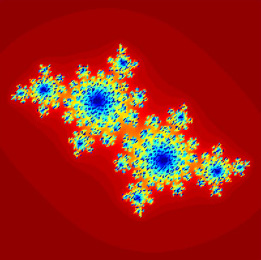
\includegraphics[scale=0.5]{images/julia.jpg}
\caption{Example of filled-in Julia set.}
\end{center}
\end{figure}

\begin{enumerate}
\item It has been shown that if the modulus of $z_n$ becomes larger than 2 for some $n$ then it is guaranteed that the orbit will tend to infinity. The value of $n$ for which this becomes true is called the 'escape velocity' of a particular $z_0$. 

Write a function that returns the escape velocity of a given $z_0$ and $c$. The function declaration should be: 
\texttt{n = escapeVelocity(z0, c, N)},
where $N$ is the maximum allowed escape velocity (basically, if the modulus of $z_n$ does not exceed 2 for $n<N$, return $N$ as the escape velocity. This will prevent infinite loops). Use \textbf{abs} to calculate the modulus of a complex number.

\item To generate the filled-in Julia Set, write the following function \texttt{M = julia(zMax, c, N)}.
$zMax$ will be the maximum of the imaginary and complex parts of the various $z_0$'s for which we will compute escape velocities. $c$ and $N$ are the same as defined above, and $M$ is the matrix that contains the escape velocity of various $z_0$'s.
\begin{itemize}
\item In this function, you first want to make a $500 \times 500$ matrix that contains complex numbers with real part between $–zMax$ and $zMax$, and imaginary part between $–zMax$ and $zMax$. 
Call this matrix $Z$. Make the imaginary part vary along the $y$ axis of this matrix. You can most easily do this by using \textbf{linspace} and \textbf{meshgrid}, but you can also do it with a loop.

\item For each element of $Z$, compute the escape velocity (by calling your \texttt{escapeVelocity}) and store it in the same location in a matrix $M$. When done, the matrix $M$ should be the same size as $Z$ and contain escape velocities with values between $1$ and $N$.

\item Run your \texttt{julia} function with various $zMax$, $c$, and $N$ values to generate various fractals.
To display the fractal nicely, use \textbf{imagesc} to visualize \texttt{atan(0.1*M)}, (taking the arctangent of $M$ makes the image look nicer; you may also want to use \textbf{axis xy} so the y values are not flipped). 

WARNING: this function may take a while to run!
\end{itemize}
\end{enumerate}

\newpage
%%%%%%%%%%%%
\Exo
\textbf{Manipulating images}\\
A color image of size $M\times N$ pixels is represented as an $M\times N \times 3$ array, where the 1st, 2nd or 3rd layers correspond respectively to the Red, Green, and Blue channels.

Write a function to display a color image, as well as its red, green, and blue layers separately. 
The function declaration should be \texttt{im = displayRGB(filename)}, where \texttt{filename} is the name of the image (make the function work for *.jpg images only), and  \texttt{im} is the final image returned as a matrix.
To test the function, you should put a jpg file into the same directory as the function and run it with the filename (include the extension, for example \texttt{im = displayRGB('testImage.jpg')}).
You can use any picture you like, from your files or off the internet. 
\begin{itemize}
\item To make the program work efficiently with all image sizes, first interpolate each color layer of the original image so that the larger dimension ends up with 800 pixels. The smaller dimension should be appropriately scaled so that the length:width ratio stays the same. 
Use \textbf{interp2} with cubic interpolation to resample the image.

\item Create a composite image that is 2 times as tall as the original, and 2 times as wide. 
Place the original image in the top left, the red layer in the top right, the green layer in the bottom left, and the blue layer in the bottom right parts of this composite image. 
The function should return the composite image matrix in case you want to save it as a jpg again (before displaying or returning, convert the values to unsigned 8-bit integers using \textbf{uint8})
\end{itemize}

Useful functions: \textbf{imread}, \textbf{meshgrid}, \textbf{interp2}, \textbf{uint8}, \textbf{image}, \textbf{axis equal}, \textbf{axis tight}.

\begin{figure}[h!]
\begin{center}
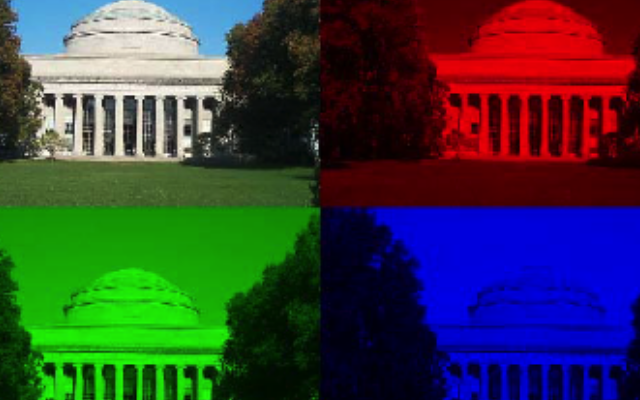
\includegraphics[scale=0.7]{images/composite.png}
\caption{Example of composite image.}
\end{center}
\end{figure}
%%%%%%%%%%%%%%%%%%%%%%%%%%%%%%%%%%%%%%%%
\end{document}
